\documentclass[11pt,letterpaper]{article}
\usepackage[hyperref]{naaclhlt2018}
\usepackage{times}
\usepackage{latexsym}

\usepackage{url}
\usepackage{latexsym}
\usepackage{subcaption}
\usepackage{amsmath}
\usepackage{multirow}
\usepackage{booktabs}
\usepackage{forest}
\forestset{
    nice empty nodes/.style={
        for tree={
            s sep=0.1em, 
            l sep=0.33em,
            inner ysep=0.4em, 
            inner xsep=0.05em,
            l=0,
            calign=midpoint,
            fit=tight,
            where n children=0{
               tier=word,
               minimum height=1.25em,
            }{},
            where n children=2{
               l-=1em,
            }{},
            parent anchor=south,
            child anchor=north,
            delay={if content={}{
                    inner sep=0pt,
                    edge path={\noexpand\path [\forestoption{edge}] 
                          (!u.parent anchor) 
                               -- (.south)\forestoption{edge label};}
                }{}}
        },
    },
}

\usepackage{url}
\usepackage{scalefnt}
\usepackage{graphicx}
\usepackage{tikz}
\usetikzlibrary{positioning}

\aclfinalcopy % Uncomment this line for the final submission
%\def\aclpaperid{***} %  Enter the acl Paper ID here

\newcommand\BibTeX{B{\sc ib}\TeX}

\title{\LaTeX~Exercises\\for DS-GA 1011}

\author{
Adina Williams$^{1}$\\
\texttt{\small adinawilliams@nyu.edu}
\And
Andrew Drozdov$^{2,}$\thanks{~~Now at eBay, Inc.} \\
\texttt{\small andrew.drozdov@nyu.edu}
\And
Samuel R.~Bowman$^{1,2,3}$\\
\texttt{\small bowman@nyu.edu}
\AND
$^{1}$\normalfont Dept. of Linguistics\\New York University\\10 Washington Place\\New York, NY 10003\And
$^{2}$\normalfont Dept. of Computer Science\\New York University\\60 Fifth Avenue\\New York, NY 10011\And
$^{3}$\normalfont Center for Data Science\\New York University\\60 Fifth Avenue\\New York, NY 10011
} 

\date{}

\begin{document}
\maketitle
\begin{abstract}
This document contains various bits and pieces pulled from a recent paper from NYU. Don't try to read it---plenty of important parts were removed to speed up compilation time. If you're curious, the actual paper is here: \url{https://arxiv.org/abs/1709.01121}. \textbf{To complete the exercises:} Open the \TeX~source for this document and look for the string ``\texttt{\% Exercise}''.
\end{abstract}

\section{Introduction}        

Tree-structured recursive neural networks \citep[TreeRNNs;][]{socher2011semi}---which build a vector representation for a sentence by incrementally computing representations for each node in its parse tree---have been proven to be effective at sentence understanding tasks like sentiment analysis \citep{socher-EtAl:2013:EMNLP}, textual entailment \citep{bowman2016spinn}, and translation \citep{eriguchi-hashimoto-tsuruoka:2016:P16-1}. Some variants of these models \citep{socher2011semi,bowman2016spinn} can also be trained to produce  parse trees that they then consume. Recent work on \textit{latent tree learning} \citep{yogatama2016learning,maillard2017jointly,choi2017unsupervised} has led to the development of new training methods for TreeRNNs that allow them to learn to parse without ever being given an example of a correct parse tree, replacing direct syntactic supervision with indirect supervision from a downstream task like sentence classification. These models are designed to learn grammars---strategies for assigning trees to sentences---that are suited to help solve the sentence understanding task at hand, rather than ones that approximate expert-designed grammars like that of the Penn Treebank \citep[PTB;][]{ptb}.
 
% Exercise 1a: Rewrite the end of the sentence above so that it renders as "Marcus et al.'s (1993) Penn Treebank." (Hint: Search for the natbib command 'citeauthor', and look for other related commands.)

% Exercise 1b: Write a new command or macro called 'cites' for "'s" constructions like this that allows you produce the same output using a single command like the one below. (Hint: Try 'newcommand')

% \cites{ptb} Penn Treebank.

\begin{figure}[t]
\centering

\begin{subfigure}[t]{\columnwidth}\centering

\scalebox{0.9}{
\begin{forest}
 shape=coordinate,
 where n children=0{
   tier=word
 }{},
 nice empty nodes
[[I] [ [saw] [[the] [ [man] [[\textbf{with}] [[\textbf{the}][\textbf{telescope}]]]]]]]
\end{forest}
}
\scalebox{0.9}{
\begin{forest}
 shape=coordinate,
 where n children=0{
   tier=word
 }{},
 nice empty nodes
[[I] [ [ [saw] [[the] [man] ] ] [[\textbf{with}] [[\textbf{the}][\textbf{telescope}]]]]]
\end{forest}
}
\caption{\footnotesize{Two different trees lead to two different interpretations for the sentence in example (\ref{tele}).}}
\end{subfigure}\\\vspace{0.5em}
\begin{subfigure}[t]{\columnwidth}\centering
\scalebox{0.9}{
\begin{forest}
 shape=coordinate,
 where n children=0{
   tier=word
 }{},
 nice empty nodes
[ [ [ [He] [swung] ] [ [at] [the] ] ] [ [ [brute] [\textbf{with}] ] [ [\textbf{his}] [, phantom ] [ [\textbf{sword}] [$.$] ] ] ] ]
\end{forest}}
\scalebox{0.9}{
\begin{forest}
 shape=coordinate,
 where n children=0{
   tier=word
 }{},
 nice empty nodes
[ [He] [ [ [ [swung] [ [at] [ [the] [brute] ] ] ] [ [\textbf{with}] [ [\textbf{his}] [\textbf{sword}] ] ] ] [$.$] ] ]
\end{forest}}%
\caption{\footnotesize{Parses generated by at ST-Gumbel model (left) and the Stanford Parser (right).}}
\end{subfigure}
 \caption{\label{fig:exampletrees} Examples of unlabeled binary parse trees.} 
\end{figure}

Latent tree learning models have shown striking success at sentence understanding, reliably performing better on sentiment analysis and textual entailment than do comparable TreeRNN models which use parses assigned by conventional parsers, and setting the state of the art among sentence-encoding models for textual entailment. However, none of the work in latent tree learning to date has included any substantial evaluation of the quality of the trees induced by these models, leaving open an important question which this paper aims to answer: Do these models owe their success to consistent, principled latent grammars?  If they do, these grammars may be worthy objects of study for researchers in syntax and semantics. If they do not, understanding why the models succeed without syntax could lead to new insights into the use of TreeRNNs and into sentence understanding more broadly.

While there is still lively debate within linguistic syntax and semantics over the precise grammars that should be used for language understanding and generation, it has been clear since at least \citet{chomskyaspects,fregesinn,kratzer1998} that understanding any natural language sentence requires implicitly or explicitly recognizing which substrings of the sentence form meaningful units or \textit{constituents}. 

This is well illustrated by syntactically ambiguous sentences like the one below, repeated from \citet{sag1991} a.o.:
\begin{enumerate}
    \item \label{tele}
    \begin{enumerate}
        \setlength\itemsep{-.25em}
        \item {I [ saw the man ] [ with the telescope ]} \\ $\hookrightarrow$ I used the telescope to view the man\label{tele1}
        \item {I saw the [ man [ with the telescope ] ]} \\ $\hookrightarrow$I saw the man who had a telescope\label{tele2}
     \end{enumerate}
\end{enumerate}

Under the constituency parse shown in \ref{tele1}, \textit{with a telescope} provides additional information about the action described by the constituent \textit{saw a man}, and in \ref{tele2}, \textit{with a telescope} provides additional information about the individual described by \textit{man}. If the same string of words can be assigned two different valid constituency structures, two different interpretations generally result. Constituency information can be straightforwardly expressed using an unlabeled parse tree like the ones used in TreeRNNs, and expressing constituency information is the generally the primary motivation for using  trees in TreeRNNs. 

In this paper, we reimplement the latent tree learning models of \citet{yogatama2016learning} and \citet{choi2017unsupervised} in a shared codebase, train both models (and several baselines) to perform textual entailment on the SNLI and MultiNLI corpora \citep{bowman-EtAl:2015:EMNLP,williams2017broad}, and evaluate the results quantitatively and qualitatively with a focus on four issues: the degree to which latent tree learning improves task performance, the degree to which latent tree learning models learn similar grammars across random restarts, the degree to which their grammars match PTB grammar, and the degree to which their grammars appear to follow any recognizable grammatical principles.

We confirm that both types of model succeed at producing useful sentence representations, but find that only the stronger of the two models---that of \citet{choi2017unsupervised}---learns a nontrivial grammar or outperforms its baseline. We find that that grammar agrees with PTB grammar with roughly chance accuracy, and does not show any other consistent, linguistically plausible patterns. We do find, though, that the resulting grammar has some regularities, including a preference for shallow trees, and a preference to treat pairs of adjacent words at the edges of a sentence as constituents.

\section{Models and Methods}

This paper investigates the behavior of two models: RL-SPINN and ST-Gumbel. Both have been shown to outperform similar models based on supervised parsing, and the two represent two substantially different approaches to latent tree learning. 

\begin{figure*}[t]
\centering
    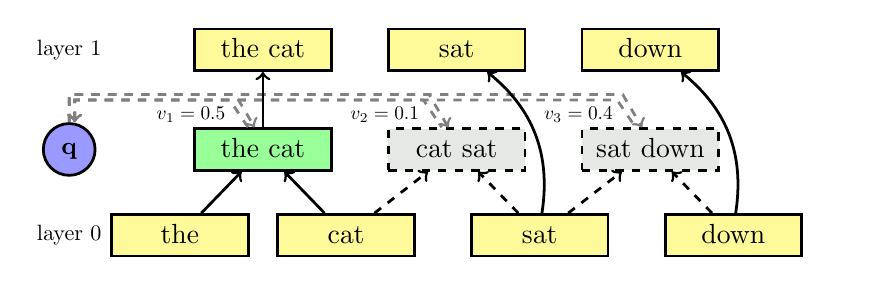
\begin{tikzpicture}[
        node distance=7em,
        every node/.style = {shape=rectangle, draw,
                             minimum height=1.5em, line width=1pt,
                             align=center, text height=2mm},
        every edge/.append style = {line width=1pt}]
    \node[text width=15mm,              fill=yellow!40] (f1) {the cat};
    \node[right of=f1, text width=15mm, fill=yellow!40] (f2) {sat};
    \node[right of=f2, text width=15mm, fill=yellow!40] (f3) {down};
    \node[left of=f1, node distance=7em, draw=none] (flabel) {\scalebox{.8}{layer 1}};
    
    \node[below=2em of f1, text width=15mm, fill=green!40] (c1) {the cat};
    \node[below=2em of f2, text width=15mm, dashed, fill=green!10!black!10] (c2) {cat sat};
    \node[below=2em of f3, text width=15mm, dashed, fill=green!10!black!10] (c3) {sat down};
    \node[right of=c3, node distance=7em, draw=none, align=left] (clabel) {\scalebox{.6}{}};
    
    \node[below=1.5em of c1, text width=15mm, xshift=-3em, fill=yellow!40] (l1) {the};
    \node[below=1.5em of c1, text width=15mm, xshift=3em, fill=yellow!40] (l2) {cat};
    \node[below=1.5em of c2, text width=15mm, xshift=3em, fill=yellow!40] (l3) {sat};
    \node[below=1.5em of c3, text width=15mm, xshift=3em, fill=yellow!40] (l4) {down};
    \node[left of=l1, node distance=4em, draw=none] (llabel) {\scalebox{.8}{layer 0}};
    
    \node[left of=c1, shape=circle, fill=blue!40] (q) {\small $\mathbf{q}$};
    \draw [->, line width=1pt, color=gray, dashed]
        (q.north)
        -- ([yshift=1em]q.north)
        -- ([xshift=6em, yshift=1em]q.north)
        -- ([xshift=-0.3em]c1.north);
    \draw [<-, line width=1pt, color=gray, dashed]
        ([xshift=0.2em]q.north)    
        -- ([xshift=0.2em,yshift=0.8em]q.north)
        -- ([xshift=5.8em, yshift=0.8em]q.north)
        -- ([xshift=-0.1em]c1);
    \node[left of=c1, node distance=2.6em, yshift=1.3em, draw=none] {\scalebox{.7}{$v_1=0.5$}};
    \draw [->, line width=1pt, color=gray, dashed]
        (q.north)
        -- ([yshift=1em]q.north)
        -- ([xshift=13em, yshift=1em]q.north)
        -- ([xshift=-0.3em]c2.north);
    \draw [<-, line width=1pt, color=gray, dashed]
        ([xshift=0.2em]q.north)    
        -- ([xshift=0.2em,yshift=0.8em]q.north)
        -- ([xshift=12.8em, yshift=0.8em]q.north)
        -- ([xshift=-0.1em]c2);
    \node[left of=c2, node distance=2.6em, yshift=1.3em, draw=none] {\scalebox{.7}{$v_2=0.1$}};
    \draw [->, line width=1pt, color=gray, dashed]
        (q.north)
        -- ([yshift=1em]q.north)
        -- ([xshift=20em, yshift=1em]q.north)
        -- ([xshift=-0.3em]c3.north);
    \draw [<-, line width=1pt, color=gray, dashed]
        ([xshift=0.2em]q.north)    
        -- ([xshift=0.2em,yshift=0.8em]q.north)
        -- ([xshift=19.8em, yshift=0.8em]q.north)
        -- ([xshift=-0.1em]c3);
    \node[left of=c3, node distance=2.6em, yshift=1.3em, draw=none] {\scalebox{.7}{$v_3=0.4$}};
    
    
    \draw [->] (c1) edge (f1);
    \draw [->] (l1) edge (c1);
    \draw [->] (l2) edge (c1);
    \draw [dashed,->] (l2) edge (c2);
    \draw [dashed,->] (l3) edge (c2);
    \draw [dashed,->] (l3) edge (c3);
    \draw [dashed,->] (l4) edge (c3);
    
    \draw [->, bend right=30] (l3) edge (f2);
    \draw [->, bend right=30] (l4) edge (f3);
    
    \end{tikzpicture}
 \caption{\label{fig:gumbel} The ST-Gumbel model in its first step of processing the sentence \textit{the cat sat down}, based on a figure by \citet{choi2017unsupervised}, used with permission. The model first computes a composed representation for every pair of adjacent words or phrases (shown with dotted lines), assigns each of these a score $v_i$, and then uses these to sample a discrete variable $q$ which determines which representation is preserved for the next layer.}
\end{figure*}

% Exercise 2a: tikz is a powerful tool for programatically drawing figures that look good in a LaTeX context. It's somewhat tricky to learn, and may not be the easiest tool for all projects, but it's worth knowing what it can do. In this exercise, we want to replace the word 'down' with 'lugubriously' (sadly) and move things around to make them fit:
% - Replace every instance of 'down' with 'lugubriously'
% - Increase the widths of the three nodes containing the new, longer, word to make it fit.
% - Adjust the arrows from the bottom row to the middle row so that they no longer overlap any nodes.
% Do your best to interpret the commands below without diving *too* deeply into the Tikz manual. You shouldn't need any new commands. Talk to your neighbor!

% Exercise 2b: You can squish figures like this into a single column to save space as long as they remain readable. Switch it to single-column mode, and shrink it to fit within the margins. (Hint: Use scalebox to shrink it. Don't shrink the caption.)

\paragraph{SPINN Variants} All three of our baselines and one of the two latent tree learning models are based on the SPINN architecture of \citet{bowman2016spinn}. 

In the base SPINN model, all model components are used, and the transition classifier is trained on binarized Penn Treebank-style parses from the Stanford PCFG Parser \citep{klein2003accurate}, which are included with SNLI and MultiNLI. These binary-branching parse trees are converted to \textsc{shift/reduce} sequences for use in the model through a simple reversible transformation.

RL-SPINN, based on the unsupervised syntax model of \citet{yogatama2016learning}, is architecturally equivalent to SPINN, but its transition classifier is optimized for MultiNLI classification accuracy, rather than any parsing-related loss. Because this component produces discrete decisions, the REINFORCE algorithm is used (with the standard moving average reward baseline) to supply gradients for it.

We also evaluate two other variants of SPINN. In SPINN-NC (for No Connection from tracking to composition), the connection from the tracking LSTM to the composition function is severed. This weakens the model, but makes it exactly equivalent to a plain TreeLSTM---it will produce the exact same vector that a TreeLSTM with the same composition function would have produced for the tree that the transition classifier implicitly produces. This model serves as a maximally comparable baseline for the ST-Gumbel model, which also performs composition using a standard TreeLSTM in forward-propagation.

SPINN-PI-NT (for Parsed Input, No Tracking) removes the tracking LSTM as well as the two components that depend on it: the tracking-composition connection and the transition decision function. As such, it cannot produce its own parse trees, and must rely on trees from the input data. We include this in our comparison to understand the degree to which training a parser, rather than using a higher-quality off-the-shelf parser, impacts performance on our semantic task.

\paragraph{ST-Gumbel}
The ST-Gumbel model was developed by \citet{choi2017unsupervised} and is shown in Figure \ref{fig:gumbel}. The model takes a sequence of $N
- 1$ steps to build a tree over $N$ words. At every step, every possible pair of adjacent words or phrase vectors in the partial tree is given to a TreeLSTM composition function to produce a new candidate phrase vector. A simple learned scoring function then selects the best of these candidates, which forms a constituent node in the tree and replaces its two children in the list of nodes that are available to compose. This repeats until only two nodes remain, at which point they are composed and the tree is complete. This exhaustive search increases the computational complexity of the model over (RL-)SPINN, but also allows the model to perform a form of easy-first parsing, making it easier for the model to explore the space of possible parsing strategies.

Though the scoring function yields discrete decisions, the Straight-Through Gumbel-Softmax estimator of \citet{jang2016categorical} makes it possible to nonetheless efficiently compute an approximate gradient for the full model without the need for relatively brittle reinforcement learning techniques. 

\paragraph{Data} Our primary experiments use the Multi-Genre Natural Language Inference Corpus \citep[MultiNLI;][]{williams2017broad}. MultiNLI is a 433k-example textual entailment dataset created in the style of SNLI, but with a more diverse range of source texts and longer and more complex sentences, which we expect will encourage the models to produce more consistent and interpretable trees than they otherwise might. Following Williams et al., we train on the combination of MultiNLI and SNLI in these experiments (yielding just under 1M training examples) and evaluate on MultiNLI (using the \textit{matched}  development and test sets). 

We also evaluate trained models on the full Wall Street Journal section of the Penn Treebank, a seminal corpus of manually-constructed constituency parses which introduced the parsing standard used in this work. Because the models under study produce and consume binary-branching constituency trees without labels (and because such trees are already included with SNLI and MultiNLI), we use the Stanford Parser's \texttt{CollapseUnaryTransformer} and \texttt{TreeBinarizer} tools to convert these Penn Treebank Trees to this form.
        
\paragraph{Sentence Pair Classification}
Because our textual entailment task requires a model to classify \textit{pairs} of sentences, but the models under study produce vectors for single sentences, we concatenate the two sentence vectors, their difference, and their elementwise product \citep[following][]{P16-2022}, and feed the result into a 1024D ReLU layer to produce a representation for the sentence pair. This representation is fed into a three-way softmax classifier that selects one of the labels \textit{entailment}, \textit{neutral}, and \textit{contradiction} for the pair.

\paragraph{Additional Details} We implement all models in PyTorch 0.2. We closely follow the original Theano code for SPINN in our implementation, and we incorporate source code provided by Choi et al.\ for the core parsing data structures and sampling mechanism of the ST-Gumbel model. Our code, saved models, and model output are available on GitHub.\footnote{\url{https://github.com/nyu-mll/spinn/tree/is-it-syntax-release}}

We use GloVe vectors to represent words \citep[standard 300D 840B word package, without fine tuning;][]{pennington2014glove}, and feed them into a $2 \times 300$D bi-directional GRU RNN (based on the \textit{leaf LSTM} of Choi et al.) to give the models access to local context information when making parsing decisions. To understand the impact of this component, we follow Choi et al.\ in also training each model with the leaf GRU replaced with a simpler context-sensitive input encoder that simply multiplies each GloVe vector by a matrix. We find that these models perform best when the temperature of the ST-Gumbel distribution is a trained parameter, rather than fixed at 1.0 as in Choi et al..

We use L2 regularization and apply dropout \citep{srivastava2014dropout} to the input of the 1024D sentence pair combination layer. We train all models using the Adam optimizer \citep{kingma2014adam}. For hyperparameters for which no obvious default value exists---the L2 and dropout parameters, the relative weighting of the gradients from REINFORCE in RL-SPINN, the starting learning rate, and the size of the tracking LSTM state in SPINN---we heuristically select ranges in which usable values can be found (focusing on MultiNLI development set performance), and then randomly sample values from those ranges. We train each model five times using different samples from those ranges and different random initializations for model parameters. We use early stopping based on development set performance with all models.


\begin{table}[t!]
\small \centering
\begin{tabular}{lcc}
\toprule
\bf Model & \bf SNLI & \bf MNLI\\
\midrule
Prior Work: Baselines & & \\
\midrule
100D LSTM (Yogatama) & 80.2 & -- \\
100D TreeLSTM (Yogatama) & 78.5 & -- \\
300D SPINN (Bowman) & 83.2 & -- \\
300D SPINN-PI-NT (Bowman) & 80.9 & -- \\
300D BiLSTM (Williams) & 81.5 & 67.5 \\
\midrule
Prior Work: Latent Tree Learning & & \\
\midrule
100D RL-SPINN (Yogatama) & 80.5 & -- \\
100D Soft Gating (Maillard) & 81.6 & -- \\
100D ST-Gumbel (Choi) & 81.9 & -- \\
\hspace{1em} w/o Leaf LSTM & 80.2 & -- \\
300D ST-Gumbel (Choi) & 84.6 & -- \\
\hspace{1em} w/o Leaf LSTM & 82.2 & -- \\
600D ST-Gumbel (Choi) & \textbf{85.4} & -- \\
\midrule
This Work: Baselines & & \\
\midrule
300D SPINN & 81.9 & 66.9  \\
\hspace{1em} w/o Leaf GRU & 82.2 & 67.5 \\ 
300D SPINN-NC & 81.6 & 68.1 \\
\hspace{1em} w/o Leaf GRU & 82.4 & 67.8 \\ 
300D SPINN-PI-NT & 81.9 & 68.2  \\
\hspace{1em} w/o Leaf GRU & 81.7 & 67.6 \\ 
\midrule
This Work: Latent Tree Learning & & \\
\midrule
300D ST-Gumbel & 83.3 & \textbf{69.5}  \\
\hspace{1em} w/o Leaf GRU & 83.7 & 67.5 \\ 
300D RL-SPINN & 81.7 & 67.3  \\
\hspace{1em} w/o Leaf GRU & 82.3 & 67.4 \\ 
\bottomrule
\end{tabular}  

% Exercise 3: Center the section headers in this table ("Prior Work: Baselines", etc.) so that they're centered with respect to the entire table, not just the left column. (Hint: Try multicolumn.)  

\caption{\label{tab:acc}Test set results. Our implementations of SPINN and RL-SPINN differ only in parser design, and our implementations of SPINN-NC and ST-Gumbel differ only in parser design. SPINN-PI-NT includes no tracking or parsing component and uses Stanford Parser trees at test time.}
\end{table}

\begin{table*}
\small
\centering
\begin{tabular}{lcccccccc}
\toprule
 & \multicolumn{2}{c}{\bf F1 wrt.} & \multicolumn{2}{c}{\bf F1 wrt.} & \multicolumn{2}{c}{\bf F1 wrt.} & \multicolumn{2}{c}{\bf Microavg.}\\
 & \multicolumn{2}{c}{\bf Left Branching} & \multicolumn{2}{c}{\bf Right Branching} & \multicolumn{2}{c}{\bf Stanford Parser}  & \multicolumn{2}{c}{\bf Depth}\\
\bf Model & $\boldsymbol{\mu~(\sigma)}$ & \bf max & $\boldsymbol{\mu~(\sigma)}$ & \bf max  & $\boldsymbol{\mu~(\sigma)}$ & \bf max  & $\boldsymbol{\mu~(\sigma)}$ & \bf max \\
\midrule
300D SPINN & 19.3 (0.4) & 19.8 & 36.9 (3.4) & \bf 42.6 & 70.2 (3.6) & \bf 74.5 & 6.2 (0.2) & 6.5 \\
\hspace{1em} w/o Leaf GRU & 21.2 (1.4) & 22.9 & 39.0 (2.6) & 41.4 & 63.5 (1.7) & 65.7 & 6.4 (0.1) & 6.5 \\
300D SPINN-NC & 19.2 (0.4) & 19.7 & 36.2 (1.4) & 38.2 & 70.5 (2.0) & 73.1 & 6.1 (0.0) & 6.1 \\
\hspace{1em} w/o Leaf GRU & 20.6 (0.5) & 21.3 & 38.9 (2.5) & 41.9 & 64.1 (2.7) & 67.1 & 6.3 (0.0) & 6.3 \\
\midrule
300D ST-Gumbel & 32.6 (2.0) & 35.6 & 37.5 (2.4) & 40.3 & 23.7 (0.9) & 25.2 & 4.1 (0.1) & 4.2 \\
\hspace{1em} w/o Leaf GRU & 30.8 (1.2) & 32.3 & 35.6 (3.3) & 39.9 & 27.5 (1.0) & 29.0 & 4.6 (0.1) & 4.7 \\
300D RL-SPINN & 95.0 (1.4) & 96.6 & 13.5 (1.8) & 15.8 & 18.8 (0.2) & 19.0 & 8.6 (0.0) & \bf 8.6 \\
\hspace{1em} w/o Leaf GRU & 99.1 (0.6) & \bf 99.8 & 10.7 (0.2) & 11.1 & 18.1 (0.1) & 18.2 & 8.6 (0.0) & \bf 8.6 \\
\midrule
Random Trees & 27.9 (0.1) & 27.9 &  28.0 (0.1) & 28.1 & 27.0 (0.1) & 27.1 & 4.4 (0.0) & 4.4 \\
\bottomrule
\end{tabular} 
\caption{\label{tab:main}\textit{F1 wrt.}~shows F1 scores on the MultiNLI development set with respect to strictly right- and left-branching trees and with respect to the Stanford Parser trees supplied with the corpus. \textit{Microavg.~Depth} shows the average across sentences of the average depth of each word in its tree. Each is shown with the mean, standard deviation, and maximum of the metric across the five runs of each model.}
\end{table*}

\section{Does latent tree learning help sentence understanding?}

Table \ref{tab:acc} shows the accuracy of all models on two test sets: SNLI (training on SNLI only, for comparison with prior work), and MultiNLI (training on both datasets). Each figure represents the accuracy of the best run, selected using the development set, of five runs with different random initializations and hyperparameter values. 

On both SNLI and MultiNLI, we reproduce the key result of Choi et al., showing that the ST-Gumbel model, which receives no syntactic information at training time, outperforms SPINN-NC, which performs composition in an identical manner but is explicitly trained to parse. This suggests that the latent trees are helpful for constructing semantic representations for sentences, whether or not they resemble conventional parse trees.

Our results with RL-SPINN are more equivocal. That model matches, but does not beat, the performance of the full SPINN model, which is equivalent except that it is trained to parse. However, our implementation of RL-SPINN outperforms Yogatama et al.'s (lower-dimensional) implementation by a substantial margin. The impact of the leaf GRU is sometimes significant, but the direction of this effect is not consistent.

Our results with SPINN-PI-NT are not substantially better than those with any other model, suggesting the relatively simple greedy parsing strategies used by the other models are not a major limiting factor in their performance. 
None of our models reach the state of the art on either task, but all are comparable in both absolute and relative performance to other published results, suggesting that we have trained reasonable examples of latent tree learning models and can draw informative conclusions by studying the behaviors of these models. 

      
\section{Analyzing the Learned Trees}

% Exercise 4: Replace 'in the previous three sections' below with 'in Section 3'. Do this without typing the number '3', so the sentence will still make sense if the section numbers change. (Hint: Use label.)

In the previous section, we have shown that latent tree learning models are able to perform as well or better than models that have access to linguistically principled parse trees at training or test time, but that the grammars that they learn are neither consistent across runs, nor meaningfully similar to PTB grammar. In this section, we investigate the trees  produced by these learned grammars directly to identify whether they capture any recognizable syntactic or semantic phenomena.

The RL-SPINN models create overwhelmingly left-branching trees. We observe few deviations from this pattern, but these occur almost exclusively on sentences of fewer than seven words.
 
In some preliminary tuning runs not shown above, we saw models that deviated from this pattern more often, and one that fixated on \textit{right}-branching structures instead, but we find no grammatically interesting patterns in any of these deviant structures. 

The ST-Gumbel models learned substantially more complex grammars, and we focus on these for the remainder of the section. We discuss three model behaviors which yield linguistically implausible constituents. The first two highlight settings where the ST-Gumbel model is consistent where it shouldn't be, and the third highlights a setting in which it is worryingly inconsistent. The models' treatment of these three phenomena and our observation of these models' behavior more broadly suggest that the models do not produce trees that follow any recognizable semantic or syntactic principles.

\section{Conclusion}

The experiments and analysis presented in this paper show that the best available models for latent tree learning learn grammars that do not correspond to the structures of formal syntax and semantics in any recognizable way. In spite of this, these models perform as well or better on sentence understanding---as measured by MultiNLI performance---as models with access to Penn Treebank-style parses.
 
This result leaves us with an immediate puzzle: What do these models---especially those based on the ST-Gumbel technique---learn that allows them to do so well? We have presented some observations, but we are left without a fully satisfying explanation. A thorough investigation of this problem will likely require a search of new architectures for sentence encoding that borrow various behaviors from the models trained in this work.

This result also opens farther-reaching questions about grammar and sentence understanding: Will the optimal grammars for sentence understanding problems like NLI---were we to explore the full space of grammars to find them---share any recognizable similarities with the structures seen in formal work on syntax and semantics? \textit{A priori}, we should expect that they should. While it is unlikely that PTB grammar is strictly optimal for any task, the empirical motivations for many of its core constituent types---the noun phrase, the prepositional phrase, and so forth---are straightforward and compelling. However, our best latent tree learning models are not able to discover these structures. 

If we accept that some form of principled constituent structure is necessary or desirable, then we are left with an engineering problem: How do we identify this structure? Making progress in this direction will likely involve both improvements to the TreeRNN models at the heart of latent tree learning systems, to make sure that these models are able to perform composition effectively enough to be able to make full use of learned structures, and also improvements to the structure search methods that are used to explore possible grammars.

\section*{Acknowledgments}

Lorem ipsum dolor sit amet, consectetuer adipiscing elit. Ut purus elit, vestibulum ut, placerat ac, adipiscing vitae, felis. Curabitur dictum gravida mauris. Nam arcu libero, nonummy eget, consectetuer id, vulputate a, magna. Donec vehicula augue eu neque. Pellentesque habitant morbi tristique senectus et netus et malesuada fames ac turpis egestas. Mauris ut leo. Cras viverra metus rhoncus sem. Nulla et lectus vestibulum urna fringilla ultrices.

\bibliographystyle{acl_natbib} 
\bibliography{exercise}

\end{document}
